\documentclass[10pt,a4paper]{article}


%==============================================================================%
% PACKAGES                                                                     %
%==============================================================================%

\usepackage{a4wide}
\usepackage{color}
\usepackage{float}
\usepackage[utf8]{inputenc}
\usepackage{lipsum}
\usepackage{listings}
\usepackage{multicol}
\usepackage{tikz}
\usetikzlibrary{arrows,shapes,positioning}


%==============================================================================%
% SETTINGS                                                                     %
%==============================================================================%

\setcounter{tocdepth}{1}

\renewcommand{\thesubsubsection}{\alph{subsubsection})}

\lstset
{
    basicstyle=\footnotesize\ttfamily,
    breaklines=true,
    frame=single,
    language=java,
    numbers=left,
    numbersep=8pt,
    tabsize=4,
}


%==============================================================================%
% DEFINITIONS                                                                  %
%==============================================================================%

\newcommand{\assignmentnumber}{2}
\newcommand{\srcroot}{../src/com/acertainbookstore/}

\newcommand{\theabstract}
{
    \lipsum[1-1]
}


%==============================================================================%
% COMMANDS                                                                     %
%==============================================================================%

% usage: \authform{<full name>}{<student id>}
\newcommand{\authform}[2]
{
    #1\\ % full name
    Department of Computer Science\\
    University of Copenhagen\\
    {\tt #2@alumni.ku.dk}\\ % student id
}

\newcommand{\colbreak}{{\ }\vfill\columnbreak}

% usage: \codeexcerpt{<file path (relative)>}{<begin line>}{<end line>}
\newcommand{\codeexcerpt}[3]
{
\begin{figure}[H]
\lstinputlisting[firstnumber=#2,firstline=#2,lastline=#3]{\srcroot/#1}
\caption{Code excerpt of {\it ../#1}, lines #2--#3}
\label{code:#1}
\end{figure}
}


%==============================================================================%
% META                                                                         %
%==============================================================================%

\title
{
    Advanced Computer Systems \\
    {\Large Assignment \assignmentnumber}
}

\author
{
    \authform{Hans J. T. Stephensen}{xkv467}
    \and
    \authform{Casper B. Hansen}{fvx507}
}

\date{\today}


%==============================================================================%
% DOCUMENT                                                                     %
%==============================================================================%

\begin{document}

\clearpage
\maketitle
\thispagestyle{empty}

\setlength{\columnsep}{0pt}
\begin{multicols}{2}
    \colbreak
    \tableofcontents
\end{multicols}
\setlength{\columnsep}{10pt}
\clearpage

%==============================================================================%
% SERIALIZABILITY & LOCKING                                                    %
%==============================================================================%

\section{Serializability \& Locking}

\begin{multicols}{2}
    ...
    \begin{figure}[H]
        \centering
        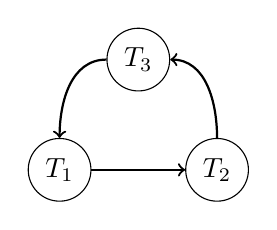
\begin{tikzpicture}
        [
            task/.style={circle, draw},
        ]
            \node[task] (T1) at (0.0, 0.0) {$T_1$};
            \node[task] (T2) at (2.0, 0.0) {$T_2$};
            \node[task] (T3) at (1.0, 1.4) {$T_3$};
            
            \draw[->, thick, draw] (T1.east) to [out=0,in=180] (T2.west);
            \draw[->, thick, draw] (T2.north) to [out=90,in=0] (T3.east);
            \draw[->, thick, draw] (T3.west) to [out=180,in=90] (T1.north);
        \end{tikzpicture}
        \caption{Precedence graph for schedule 1}
        \label{fig:trans-schedule-1}
    \end{figure}
    Since the graph forms a cycle, schedule 1 is not conflict serializable.

    \colbreak

    ...
    \begin{figure}[H]
        \centering
        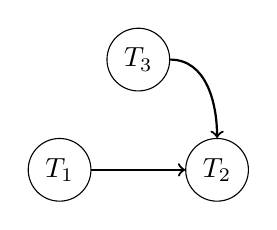
\begin{tikzpicture}
        [
            task/.style={circle, draw},
        ]
            \node[task] (T1) at (0.0, 0.0) {$T_1$};
            \node[task] (T2) at (2.0, 0.0) {$T_2$};
            \node[task] (T3) at (1.0, 1.4) {$T_3$};
            
            \draw[->, thick, draw] (T1.east) to [out=0,in=180] (T2.west);
            \draw[->, thick, draw] (T3.east) to [out=0,in=90] (T2.north);
        \end{tikzpicture}
        \caption{Precedence graph for schedule 2}
        \label{fig:trans-schedule-2}
    \end{figure}

\end{multicols}

%==============================================================================%
% OPTIMISTIC CONCURRENCY CONTROL                                               %
%==============================================================================%

\section{Optimistic Concurrency Control}
...

%==============================================================================%
% DISCUSSION                                                                   %
%==============================================================================%

\section{Discussion on the Performance Measurements}
...

\subsection{Setup}
\dots

\subsection{Plots}
\dots

\subsection{Reliability}
\dots


\end{document}
